\documentclass[a4paper,12pt]{article}

\usepackage{hyperref}
\usepackage{cmsrb}
\usepackage[T1]{fontenc}
\usepackage[serbian]{babel}
\usepackage[utf8]{inputenc}
\usepackage{csquotes}
\usepackage{lmodern}
\usepackage{graphicx}
\usepackage{caption}
\usepackage[
	backend=biber,
	style=alphabetic,
	sorting=ynt
]{biblatex}
\addbibresource{citation.bib}
\usepackage{amsmath}
\usepackage{amsfonts}
\usepackage{float}

\hypersetup{
	colorlinks,
	citecolor=black,
	filecolor=black,
	linkcolor=black,
	urlcolor=black
}

\renewcommand{\contentsname}{Sadržaj}

\title{Automatsko prepoznavanje teksta sa tablica automobila koristeći Jedinstveni Vizuelni Model za Prepoznavanje Teksta na Sceni}
\date{}
%\author{Student: {\normalfont Andrija Urošević} \\ \newline Mentor: {\normalfont dr Nemanja Ilić}}

\begin{document}
	\emergencystretch 3em
	\begin{titlepage}
		\pagenumbering{gobble} % Remove page numbering
		\centering
		{\huge\bfseries \maketitle}
		
		{\large
			\textbf{Student:}
			Andrija Urošević
			\par
%			\hspace{0.7cm}
			\bigskip
			\textbf{Mentor:}
			dr Nemanja Ilić
		}
	
		\vfill
		{\large Računarski fakultet,\par}
		{\large Univerzitet Union\par}
		\bigskip
		\date{Jul 2024}
	\end{titlepage}
	
	\pagenumbering{roman}
	
	\section*{Predgovor}
	\addcontentsline{toc}{section}{Predgovor}
	Prostor za predgovor.
	\newpage
	
	\tableofcontents
	\newpage
	
	\pagenumbering{arabic}
	
	\section*{Sažetak}
	\addcontentsline{toc}{section}{Sažetak}
	\noindent
	Automatsko prepoznavanje teksta sa registarskih tablica automobila od izuzetne je važnositi za savremene sisteme nadzora saobraćaja, praćenje vozila i obezbeđenje sigurnosti na putevima. Identifikacija registarskih tablica ima različite primene, uključujući praćenje ukradenih vozila, naplatu putarine, sigurnosne provere i nadzor saobraćaja. U proteklim decenijama, napredak u oblasti obrade slike i mašinskog učenja omogućio je razvoj efikasnih sistema za automatsko prepoznavanje teksta sa tablica vozila. Primena dubokih neuronskih mreža i algoritama dubokog učenja omogućila je visoku tačnost prepoznavanja teksta, čak i u složenim scenama i različitim uslovima snimanja. Ovaj rad istražuje metode i tehnike za automatsko prepoznavanje teksta sa tablica automobila, sa ciljem razvoja sistema koji može precizno identifikovati registarske tablice u realnom vremenu. Eksperimentalni rezultati prikazuju performanse sistema u stvarnim uslovima i ukazuju na mogućnosti za primenu u različitim oblastima, uključujući nadzor saobraćaja, bezbednosne provere i identifikaciju vozila.
	\newpage
	
	\section{Uvod}
	Automatsko prepoznavanje teksta je ključna tehnologija u oblasti kompjuterske vizije koja ima široku primenu u različitim aplikacijama, uključujući prepoznavanje registarskih tablica vozila, prepoznavanje rukopisa, prepoznavanje dokumenata i mnoge druge. Glavni cilj automatskog prepoznavanja teksta je pretvaranje vizuelno prikazanog teksta u format koji računari mogu razumeti i obrađivati, omogućavajući im da interpretiraju tekstualne informacije slično kao što to radi čovek.
		
	Automatsko prepoznavanje teksta sa registarskih tablica automobila obuhvata nekoliko ključnih koraka koji se odvijaju u procesu od prikupljanja podataka do konačne integracije sistema u softver za prepoznavanje tablica automobila.
	
	Prikupljanje raznovrsnog skupa slika registarskih tablica vozila ključno je za uspešno treniranje modela. Ove slike treba da obuhvataju različite tipove tablica, različite uslove osvetljenja i pozadine kako bi model bio što robustniji. Nakon prikupljanja, slike treba pažljivo razvrstati na one koje su pogodne za treniranje modela i one koje nisu. Ovo uključuje filtriranje slika sa veoma lošim kvalitetom, zamućenim ili nejasnim tablicama. Kako bi se obogatio skup podataka i poboljšala generalizacija modela, potrebno je primeniti tehnike augmentacije podataka. Ovo uključuje manipulaciju sa slikama kao što su rotacija, promena osvetljenja, izobličenja i dodavanje šuma. Pored toga, sintetički podaci se mogu generisati korišćenjem programa za generisanje tablica sa tekstom. Svaka slika mora biti precizno označena sa tačnim tekstualnim sadržajem registarske tablice kako bi se koristila za obuku modela. Ovaj proces može biti ručan ili se može koristiti alat za automatsko lejbelovanje. Nakon pripreme podataka, sledi faza treniranja mreže za prepoznavanje teksta. U ovoj fazi, model se obučava nad označenim podacima kako bi naučio da prepoznaje tekst sa slika tablica. Kada je model obučen, integriše se u softver za prepoznavanje tablica automobila. Ovaj softver obično obuhvata module za detekciju tablica, detekciju teksta na tablicama, formatiranje izlaza i druge funkcionalnosti.
	
	Kako bi omogućili portabilnost i lakšu distribuciju sistema za prepoznavanje tablica, koristi se Docker kontejner. Docker omogućava pakovanje softverskih aplikacija i njihovo pokretanje u izolovanim okruženjima. Još jedna od bitnih komponenata je Python web framework - FastAPI koji omogućava brzo kreiranje API-ja za komunikaciju sa softverskim komponentama. Integracija Docker-a i FastAPI modula omogućava da se servis za prepoznavanje teksta koristi nezavisno od platforme na kojoj se izvršava, čineći ga pristupačnim i jednostavnim za upotrebu u različitim okruženjima.
	\newpage
	
	\section{Prepoznavanje teksta}
	\subsection{Uvod u prepoznavanje teksta}
	Prepoznavanje teksta na sceni ima za cilj da tekst sa slika konvertuje u digitalni niz karaktera, što prenosi semantiku visokog nivoa ključnu za razumevanje scene. Zadatak prepoznavanja teksta sa scene je izazovan zbog varijacija u: deformacijama teksta, fontovima, preklapanjima različitih tekstova, prekompleksnim pozadinama, itd. Dodatno, otežavajući faktor može biti i to što se tekst može pojaviti pod različitim uglovima.
	
	\begin{figure}[H]
		\centering
		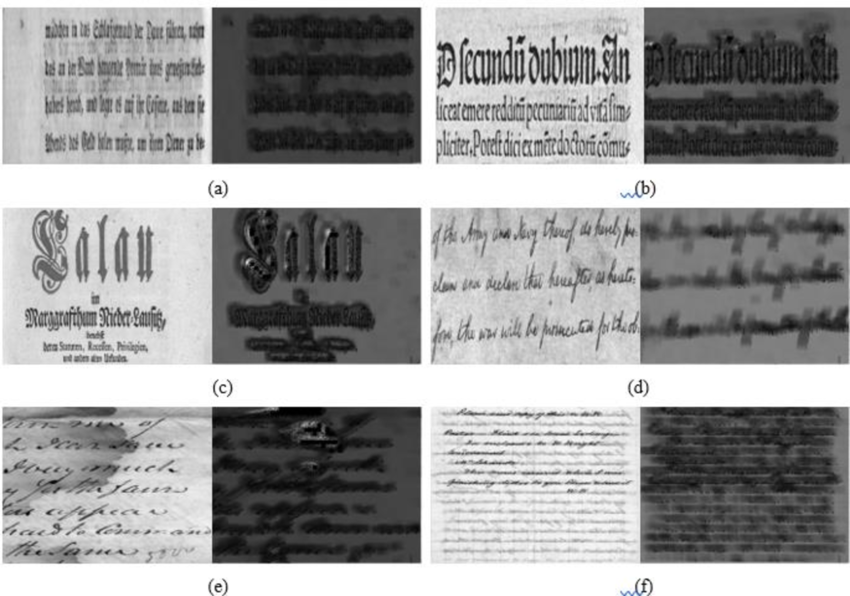
\includegraphics[width=\textwidth]{assets/text.png}
		\caption{Tekst na sceni sa različitim fontovima, pozadinama, osvetljenjem i slično}
		\label{fig:text-on-scene}
	\end{figure}
	
	U proteklim godinama uloženi su brojni napori kako bi se poboljšala tačnost prepoznavanja teksta. Moderni pristupi za prepoznavanje teksta, pored tačnosti, takođe uzimaju u obzir i faktore poput brzine izvršavanja modela zbog praktičnih zahteva.
	
	Metodološki, prepoznavanje teksta na sceni može se posmatrati kao prelazak iz modaliteta slike u niz karaktera. Obično, prepoznavanje teksta se sastoji od dva osnovna dela, vizuelnog modela za ekstrakciju karakteristika i sekvencijskog modela za transkripciju teksta.
	\newpage
	
	\subsection{Istorijski pregled prepoznavanja teksta}
	
	Prvi primeri i prva faza tehnologije optičkog prepoznavanja karaktera(OCR) pojavili su se sredinom 20. veka, pretežno tokom 1950-ih i 1960-ih godina. Ovo doba obeležilo je razvoj ranih sistema OCR-a, koji su koristili osnovne tehnike prepoznavanja obrazaca kako bi prepoznali mašinski odštampane karaktere. Ovi sistemi su često bili ograničeni na prepoznavanje određenih fontova i imali su relativno nisku stopu tačnosti u poređenju sa modernom OCR tehnologijom. Glavna primena im je bila čitanje standardizovanih obrazaca i dokumenata sa jasno štampanim tekstom i poznatim fontom.
	
	Druga faza tehnologije optičkog prepoznavanja karaktera dogodila se krajem 20. veka i početkom 21. veka, počevši oko 1970-ih i nastavljajući se u 2000-ima. Ovo doba je obeleženo značajnim napretkom u tehnologiji OCR-a, uključujući razvoj sofisticiranih algoritama i tehnika za prepoznavanje karaktera. Ovi napredci doveli su do veće tačnosti i mogućnosti prepoznavanja šireg spektra fontova, jezika i rasporeda dokumenata. Dodatno, integracija pristupa mašinskog učenja i neuronskih mreža doprinela je daljem poboljšanju performansi OCR-a. U ovoj fazi došlo je do primene OCR sistema u širem spektru aplikacija, od skeniranja i konverzije dokumenata u digitalno arhiviranje, do automatizovanog unosa podataka i ekstrakcije teksta u različitim industrijama.
	
	Treća faza tehnologije optičkog prepoznavanja karaktera je trenutno aktuelna i predstavlja trenutno stanje napretka u sistemima OCR-a. Ovo doba karakteriše integracija najnovijih tehnologija poput dubokog učenja, konvolucionih neuronskih mreža (CNN) i rekurentnih neuronskih mreža (RNN) u algoritme OCR-a. Ove napredne tehnike značajno su poboljšale tačnost i pouzdanost sistema OCR-a, omogućavajući prepoznavanje složenih dokumenata sa različitim fontovima, rasporedima i jezicima. Osim toga, pojava OCR usluga zasnovanih na cloud-u i integracija OCR funkcionalnosti u mobilne uređaje učinili su OCR dostupnijim i svestranijim nego ikad ranije. Treća faza takođe obuhvata napretke u analizi i razumevanju dokumenata, omogućavajući OCR sistemima da izvlače ne samo tekst već i strukturalne i semantičke informacije iz dokumenata, što dovodi do poboljšanih sposobnosti obrade dokumenata i pretraživanja informacija.
	
	\subsection{Arhitekture modela za prpoznavanje teksta na slici}
	
	\begin{figure}[H]
		\centering
		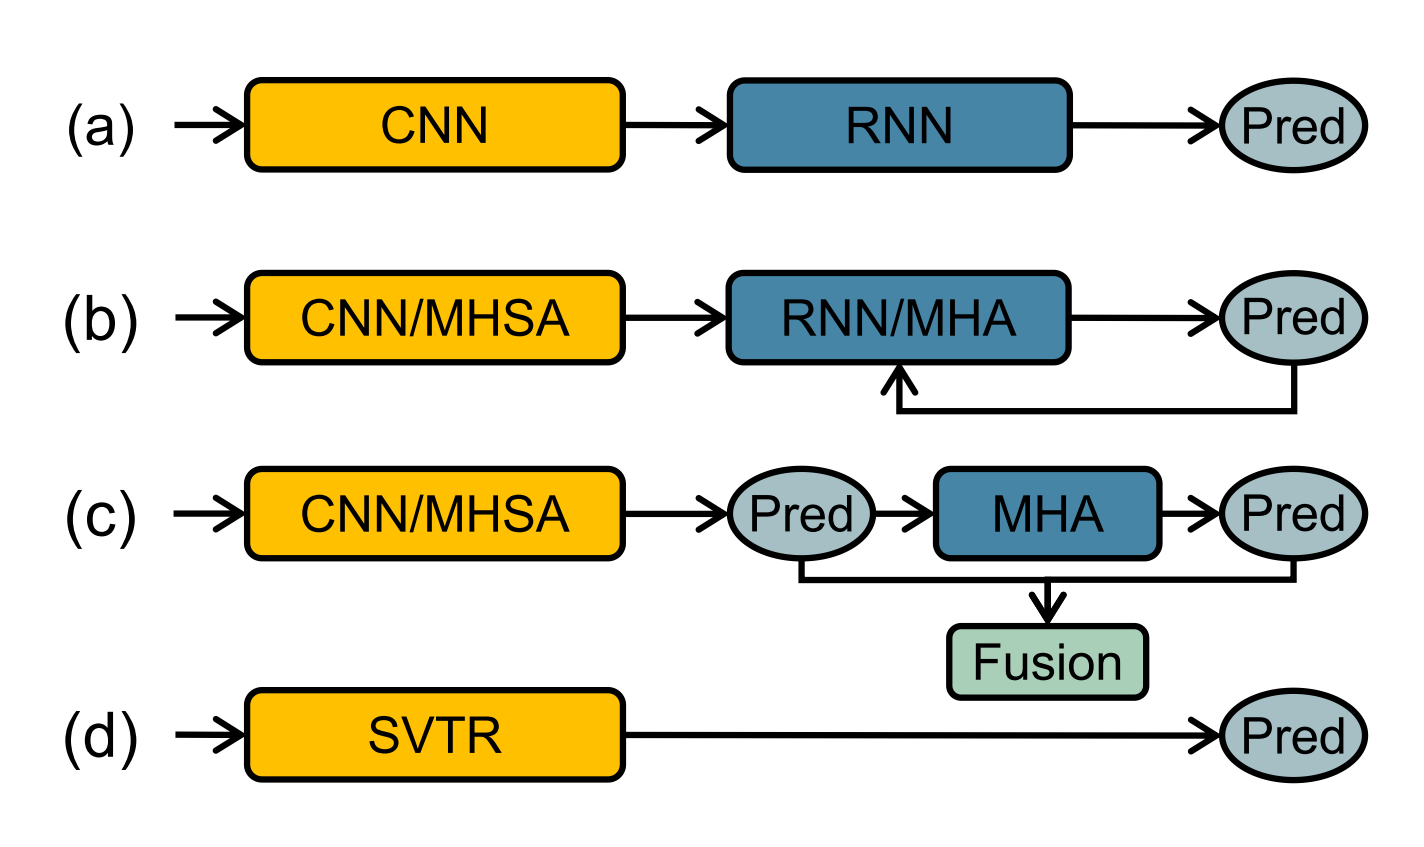
\includegraphics[width=\textwidth]{assets/text-recognition-model-architectures.png}
		\caption{Arhitekture modela za prepoznavanje teksta sa scene. (a) Modeli zasnovani na CNN-RNN. (b) Modeli kodiranja-dekodiranja. (c) Vizuelno-jezički modeli. (d) SVTR, koji prepoznaje tekst scene sa jedinstvenim vizuelnim modelom i odlikuje se efikasnošću, tačnošću i višejezičnom svestranošću.}
		\label{fig:tr-model-architectures}
	\end{figure}
	
	Modeli zasnovani na CNN-RNN \cite{shi2015endtoend} prvo koriste CNN za ekstrakciju karakteristika. Karakteristike se zatim preoblikuju u sekvencu koju BiLSTM modeluje uz pomoć CTC gubitka kako bi generisao predikciju (Slika \ref{fig:tr-model-architectures}(a)). Odlikuju se efikasnošću i ostaju izbor za neke komercijalne proizvode za prepoznavanje teksta sa scene. Međutim, preoblikovanje karakteristika u sekvencu je osetljivo na deformacije teksta, što ograničava efikasnost takvih modela.
	
	Kasnije su pristupi zasnovani na auto-regresivnim metodama kodera-dekodera postale popularne \cite{sheng2019nrtr, li2019show, zheng2023cdistnet}. Ove metode transformišu prepoznavanje u iterativni proces dekodiranja (Slika \ref{fig:tr-model-architectures}(b)). Kao rezultat, postignuta je poboljšana tačnost jer je uzeta u obzir kontekstualna informacija. Međutim, brzina izvođenja je spora zbog transkripcije karakter po karakter. Ovaj postupak je dodatno proširen na softversku strukturu zasnovanu na viziji i jeziku \cite{yu2020accuratescenetextrecognition, fang2021readlikehumansautonomous}, gde je jezičko znanje uključeno (Slika \ref{fig:tr-model-architectures}(c)) i sprovedena je paralelna predikcija. Ipak, ovaj postupak često zahteva model sa velikim kapacitetom ili složenu paradigmu prepoznavanja kako bi se osigurala tačnost prepoznavanja, što ograničava njegovu efikasnost.
	
	U poslednje vreme, naglasak je na razvoju pojednostavljenih arhitektura kako bi se dobilo na brzini izvršavanja. Na primer, korišćenje složene paradigme obuke, ali jednostavnog modela za izvršavanje. Rešenje zasnovano na CRNN-RNN ponovo je pregledano u sledećem radu: \cite{Hu_Cai_Hou_Yi_Lin_2020}. Koristi mehanizam pažnje i grafovsku neuronsku mrežu za agregaciju sekvencijalnih karakteristika koje odgovaraju istom karakteru. Pri izvršavanju, deo za modelovanje zasnovan na mehanizmu pažnje je odbačen kako bi se uskladila tačnost i brzina.
	
	Nedavni uspeh transformera za obradu slike \cite{dosovitskiy2021imageworth16x16words, liu2021swintransformerhierarchicalvision}, inspirisao je nastanak jedinstvenog vizuelnog modela za prepoznavanje teskta na sceni(SVTR) \cite{du2022svtrscenetextrecognition}. SVTR najpre razlaže tekst slike na male 2D isečke koji se nazvaju komponente karaktera, od kojih svaka komponenta može sadržati samo deo karaktera. Tokenizacija slike po isečcima praćena mehanizmom samopažnje se primenjuje da bi se uhvatile indicije prepoznavanja teksta među komponentama karaktera. Za ovu svrhu je razvijena prilagođena arhitektura za tekst, čija osnovna struktura sadrži progresivno smanjujuću visinu mape karakteristika u tri faze i uključujue operacije mešanja, spajanja i/ili kombinovanja. Osmišljeni su lokalni i globalni blokovi mešanja koji se rekurzivno primenjuju u svakoj fazi, zajedno sa operacijom spajanja ili kombinovanja, stičući tako afinitete na nivou lokalnih komponenti koje predstavljaju karakteristike slične potezima karaktera i dugoročne zavisnosti između različitih karaktera. Dakle, osnovna struktura ekstraktuje karakteristike komponenti na različitim rastojanjima i na više skala, formirajući višeslojnu percepciju karakteristika karaktera. Kao rezultat, prepoznavanje teksta se postiže jednostavnom linearnom predikcijom. U celom procesu koristi se samo jedan vizuelni model (Slika \ref{fig:tr-model-architectures}(d)).

	\subsection{Korišćenje Jedinstvenog Vizuelnog Modela za Prepoznavanje Teksta na Sceni}
	
	Tradicionalni modeli za prepoznavanje teksta obično uključuju dve odvojene komponente: vizuelni model za izdvajanje karakteristika sa slike i sekvencijalni model za dekodiranje izdvojenih karakteristika u tekst. Jedinstveni vizuelni model za prepoznavanje teksta na sceni(SVTR) eliminiše potrebu za sekvencijalnim modelom u potpunosti, čineći ga jednostavnijim i efikasnijim.
	
	Uklanjanjem komponente sekvencijalnog modeliranja, SVTR postiže konkurentnu preciznost na zadacima prepoznavanja teksta, pružajući veću efikasnost u poređenju sa tradicionalnim metodama.
	
	\subsubsection{Arhiterktura}

	Pregled SVTR modela je prikazan na (Slika \ref{fig:svtr-architecture}) i predstavlja tro-faznu mrežu sa progresivno smanjujućom visinom, namenjenu za prepoznavanje teksta. Slika teksta veličine H×W×3, prvo se transformiše u \(\dfrac{H}{4} \times \dfrac{W}{4}\) isečaka dimenzije \(D_0\) koristeći progresivno preklapajuće ugrađivanje isečaka. Isečci predstavljaju karakterne(znakovne) komponente, od kojih svaka odgovara delu tekstualnog karaktera na slici. Zatim se izvode tri faze, od kojih se svaka sastoji od niza blokova za mešanje praćenih operacijom spajanja ili kombinovanja, na različitim skalama za ekstrakciju karakteristika. Osmišljeni su lokalni i globalni blokovi za mešanje za ekstrakciju lokalnih obrazaca nalik potezima i hvatanje međukomponentne zavisnosti. Pomoću osnovne strukture se karakterizuju komponentne karakteristike i zavisnosti na različitim udaljenostima i na više skala, predstavljene kao C veličine \(1 \times \dfrac{W}{4} \times D_3\), koje percipira karakteristike znakova na više nivoa granularnosti. Na kraju procesa, model istovremeno predviđa sve znakove sa ulazne slike i primenjuje postupak uklanjanja duplikata kako bi se eliminisali eventualno pogrešno ponovljeni karakteri koje je model predvideo, a koji nisu stvarno prisutni na originalnoj slici. Rezultat ovog procesa je konačan niz prepoznatih znakova.

	\begin{figure}[H]
		\centering
		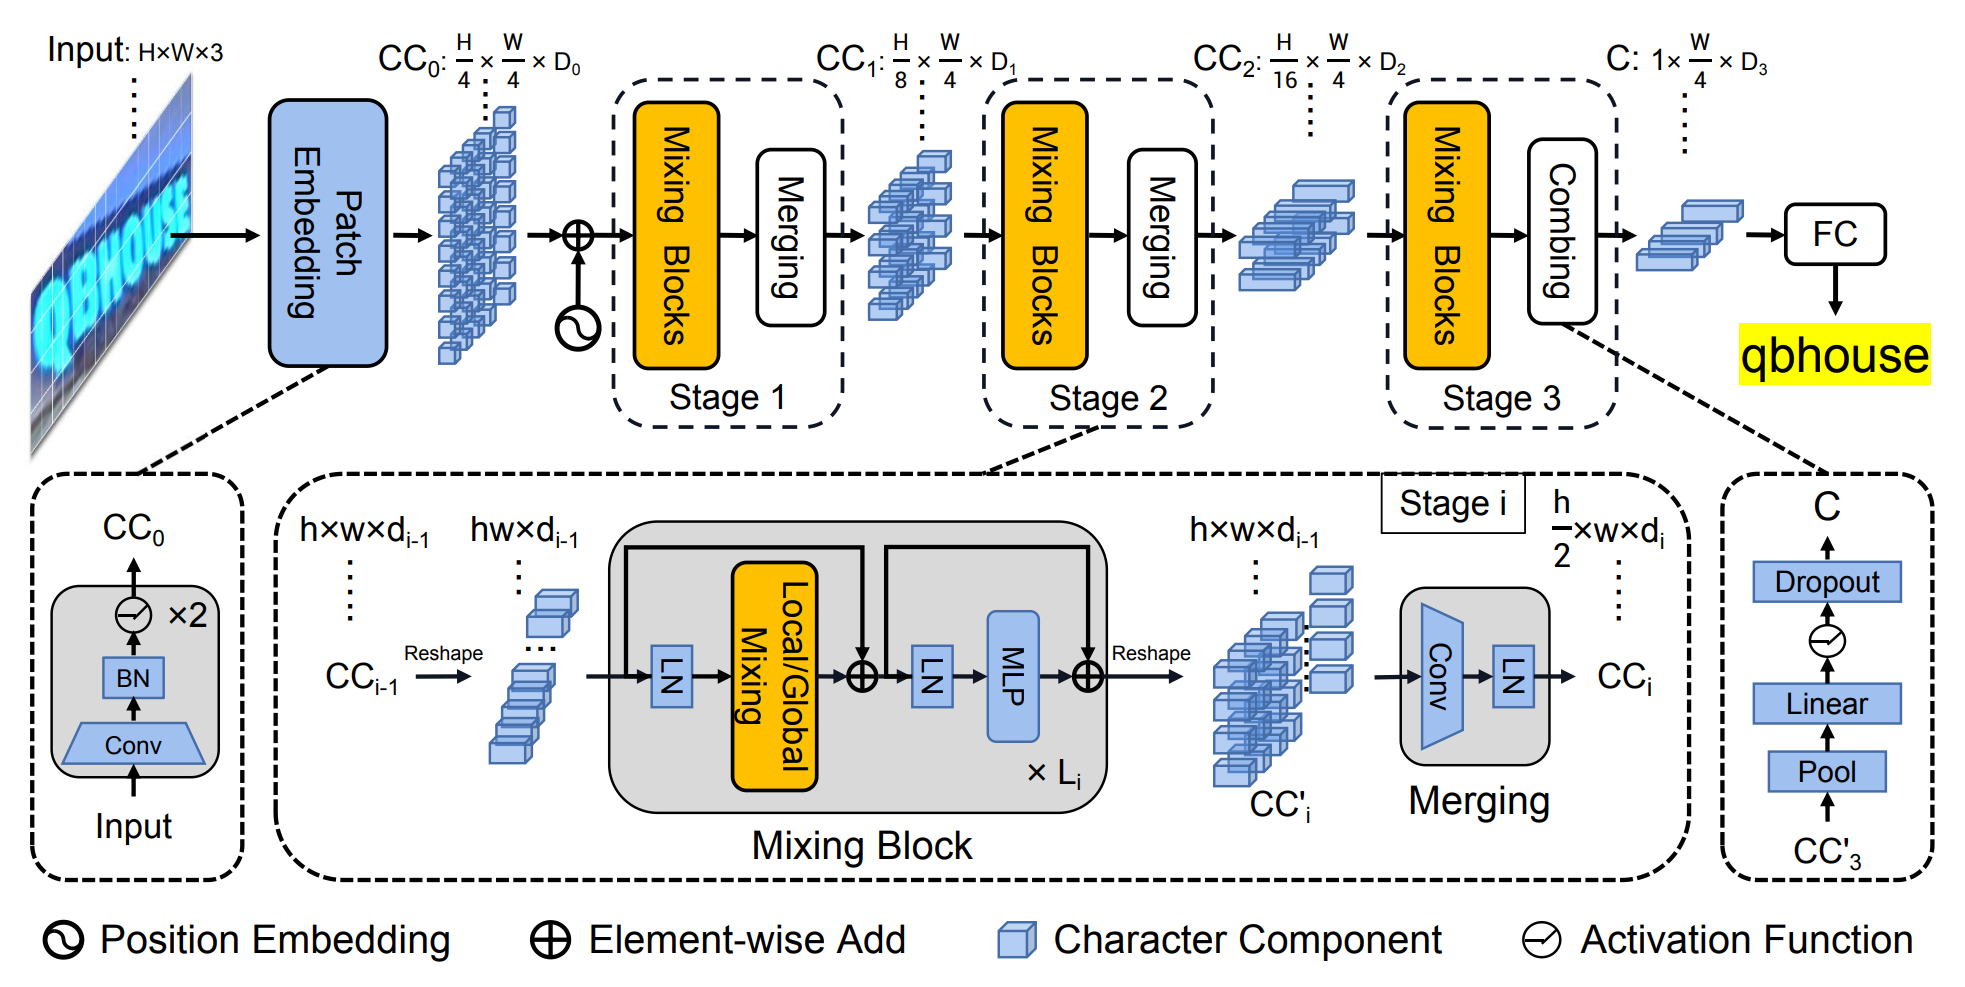
\includegraphics[width=\textwidth]{assets/svtr-architecture.png}
		\caption{Arhitektura SVTR-a: Mreža koja kroz tri faze progresivno smanjuje visinu mape karakteristika. U svakoj fazi se izvodi niz blokova za mešanje, nakon čega sledi operacija spajanja ili kombinovanja. Na kraju se prepoznavanje vrši linearnim predviđanjem.}
		\label{fig:svtr-architecture}
	\end{figure}
	
	\subsubsection{Progresivno preklapajuće ugrađivanje isečaka}
	
	Pvri korak u obradi slike teksta je njeno razlaganje na manje delove koje nazivamo isečcima. Dobijanje karakterističnih isečaka koji predstavljaju komponente znakova znači prelazak iz \(X \in \mathbb{R}^{H \times W \times D_0}\) u \(CC_0 \in \mathbb{R}^{\dfrac{H}{4} \times \dfrac{W}{4} \times D_0}\). Postoje dva uobičajena načina da se ovo uradi — korišćenje \(4 \times 4\) mreže za podelu slike i linearna transformacija svakog dela(Slika \ref{fig:linear-projection-in-ViT}(a)) i korišćenje \(7 \times 7\) konvolucionog filtera sa korakom 4. Autori SVTRa su izabrali alternativni metod. Oni koriste dva manja konvoluciona filtera \(3 \times 3\) jedan za drugim sa korakom 2, kao što je prikazano na (Slika \ref{fig:linear-projection-in-ViT}(b)). Takođe koriste tehniku zvanu normalizacija serije da bi održali brojeve pod kontrolom. Ovaj novi metod zahteva nešto više računarske snage, ali je bolji u kombinovanju karakteristika iz slike.

	\begin{figure}[H]
		\centering
		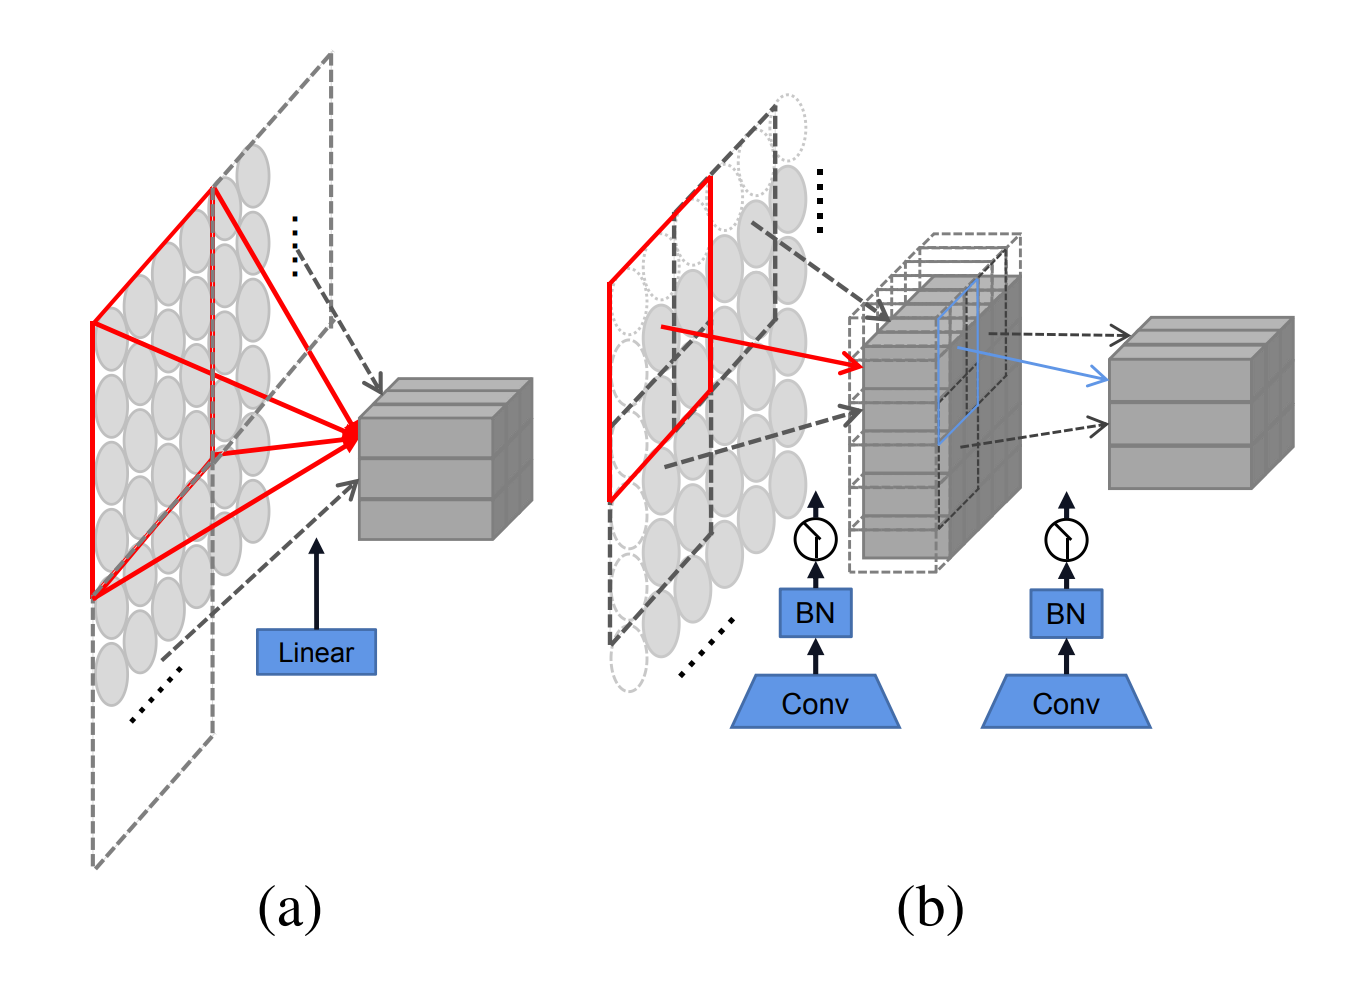
\includegraphics[width=\textwidth]{assets/linear-projection-in-ViT.png}
		\caption{(a) Linearna projekcija u ViT \cite{dosovitskiy2021imageworth16x16words}. (b) SVTR progresivno preklapajuće ugrađivanje isečaka.}
		\label{fig:linear-projection-in-ViT}
	\end{figure}
	
	\subsubsection{Blok mešanja}
	
	S obzirom na to da se dva karaktera mogu blago razlikovati važno je posmatrati male delove koji čine karaktere. Prepoznavanje teksta se u velikoj meri oslanja na ekstrakciji karakteristika na nivou komponenti karaktera. Međutim, postojeće studije uglavnom koriste niz karakteristika za predstavljanje teksta na slici. Svaka karakteristika odgovara deliću regiona slike, koji je često nerazumljiv, posebno za nepravilan tekst — što nije optimalno za opisivanje karaktera. Nedavni napredak u vizuelnim transformatorima uvodi 2D reprezentaciju karakteristika, ali njeno korišćenje u kontekstu prepoznavanja teksta je još uvek u fazi istraživanja. Autori SVTRa sugerišu da su dve vrste karakteristika važne za prepoznavanje teksta. Prva su lokalni obrasci, kao što su mali detalji koji čine karakter, poput poteza. Oni pokazuju kako su različiti delovi karaktera međusobno povezani i stvaraju se morfološke karakteristike i korelacije između različitih delova karaktera. Druga su međukarakterne zavisnosti, koje se odnose na to kako su različiti karakteri povezani jedni s drugima, ili kako se tekst odnosi na netekstualne delove slike. Da bi uhvatili ove karakteristike, autori su kreirali dva posebna bloka mešanja. Ovi blokovi koriste tehniku zvanu samopažnja, koja pomaže modelu da se fokusira na važne delove slike. Koristeći dva različita područja fokusa koja mehanizam samopažnje razmatra, ovi blokovi mogu uhvatiti i male detalje i širu sliku o tome kako su karakteri međusobno povezani.
	\newpage
	
	\section{Primene}
%	Slanje upozorenja za parking
	\newpage
	
	\section{Prikupljanje i rad sa podacima}
	\subsection{Upoznavanje sa podacima}
	\subsection{Augmentacija podataka}
	\subsection{Razvrstavanje i čišćenje podataka}
	\subsection{Pravljenje sintetičkog data seta}
	\subsubsection{Generisanje pozadina tablica}
	\subsubsection{Generisanje teskta na tablicama}
	\newpage
	
	\section{Implementacija}
	\subsection{Treniranje modela prepoznavanja teksta}
	\subsection{Komponente sistema}
	\subsubsection{Detektor tablica}
	\subsubsection{Detektor teksta}
	\subsubsection{Prepoznavanje teksta}
	\subsection{Tehnologije}
	\subsubsection{PaddlePaddle}
	\subsubsection{Docker}
	\subsubsection{FastAPI}
	\newpage
	
	\section{Rezultati}
	\newpage
	
	\section{Buduća poboljšanja}
	\newpage
	
	\section{Zaključak}
	\newpage
	
	\printbibliography
	\addcontentsline{toc}{section}{Literatura}
\end{document}